\documentclass[0-main.tex]{subfiles}
\begin{document}


\section{Introduction}
Segmentation is an important first step in robot learning from complex demonstrations, and it has been applied to skill-learning \cite{calinon2010learning, kruger2010learning, konidaris2011robot}, learning from demonstrations \cite{Niekum2015learning}, reward function parametrization \cite{hanlearning}, and automation of surgical subtasks \cite{murali2015learning}.
Manual annotation is one approach; however, this can be time-consuming and error-prone if inconsistent.
There are a number of recent proposals to algorithmically extract segments from unlabeled data.
Such algorithms fall into two broad categories: (1) dictionary-based, (2) and unsupervised.
Dictionary-based algorithms construct a pre-defined vocabulary of primitives \emph{a priori} and decompose new trajectories in terms of the primitives.
However, the key challenge in using a dictionary-based approach is building the dictionary of primitives. 
Narrowly specified primitives may not cover all of the actions seen in a set of demonstrations, while broad primitives may miss task-specific structure.

\begin{figure}[t!]
\centering
\vspace{-5pt}
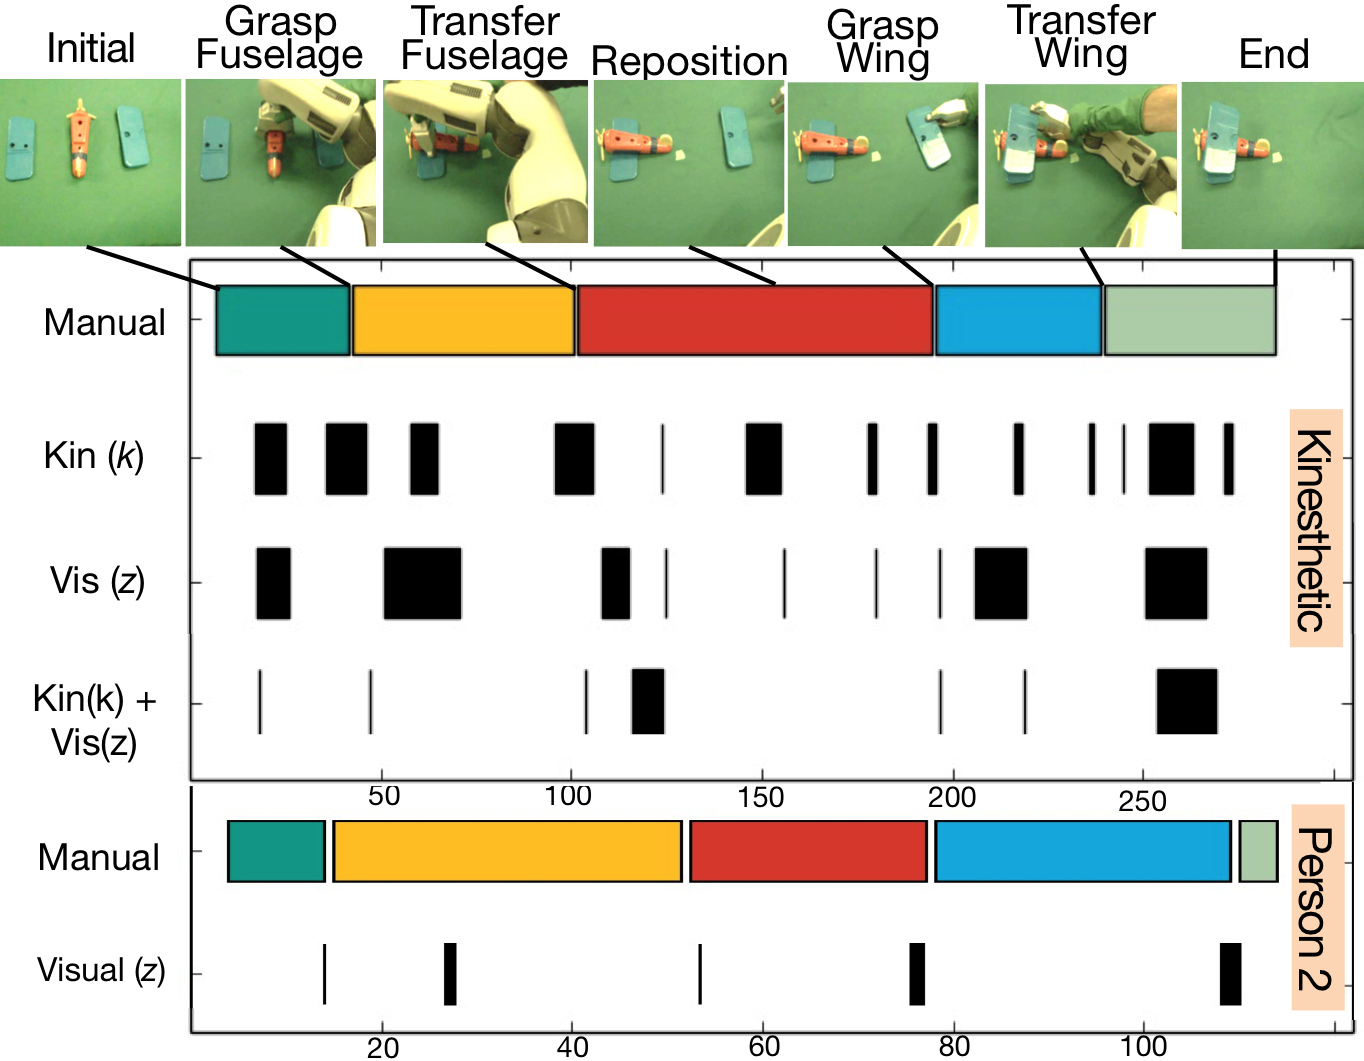
\includegraphics[width=\linewidth]{figures/pr2_plane_assembly.png}
\caption{The figure displays a sequence of images from partial assembly of a Toy Plane (YCB Dataset). The first row shows a manual segmentation of the task in 4 semantic steps: Grasp Fuselage, Transfer Fuselage, Grasp Wing, Transfer Fuselage. Rows 2-4 exhibit the sub-task level segmentation learned by our \del{completely} unsupervised approach using 8 demonstrations. Each row is a sequence of transitions represented by blocks. The width of each block represents the confidence interval conveying the length of transition, with some transitions being near instantaneous while others are gradual.\todo{label figure}}
\figlabel{pr2_toyplane}
% \label{fig:pr2_toyplane}
\vspace{-15pt} 
\end{figure}


\begin{SCfigure*}[][t!]
    \centering
    \vspace{-10pt}
    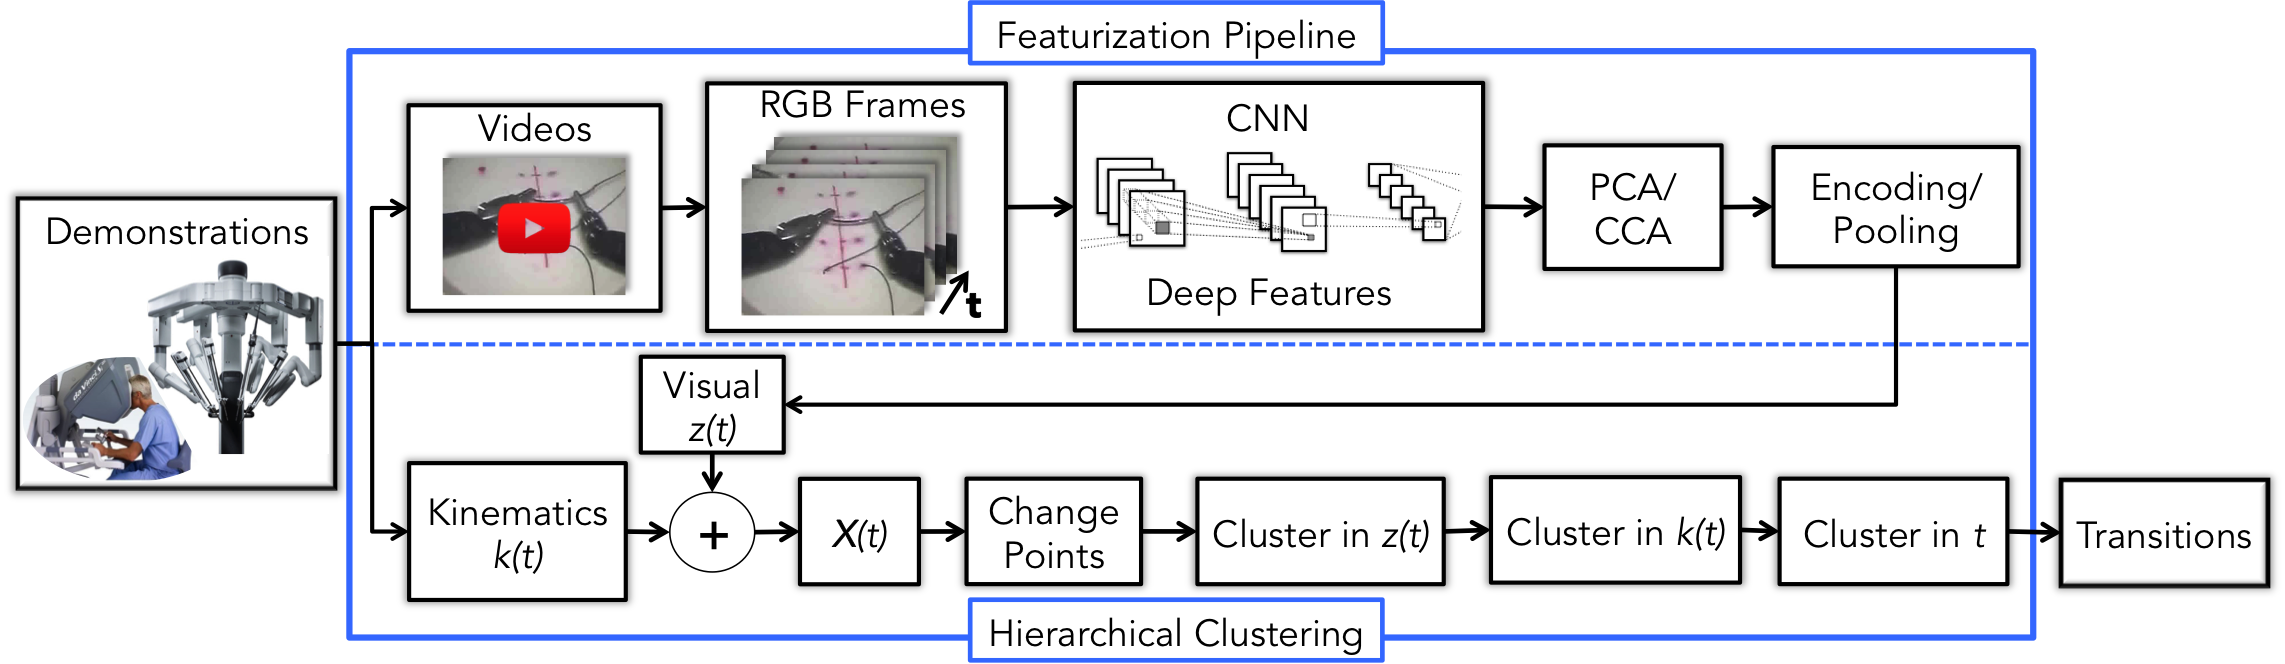
\includegraphics[width=1.5\linewidth]{figures/sysArch}
    \caption{\tsc is a task segmentation pipeline that starts with multimodal demonstrations (kinematics and vision), uses deep learning to featurize the frames of the video, and then clusters transition events to find segments.}
    \label{fig:pipeline}
    \vspace{-10pt}
\end{SCfigure*}

% \begin{figure*}[!t]
% \centering
% 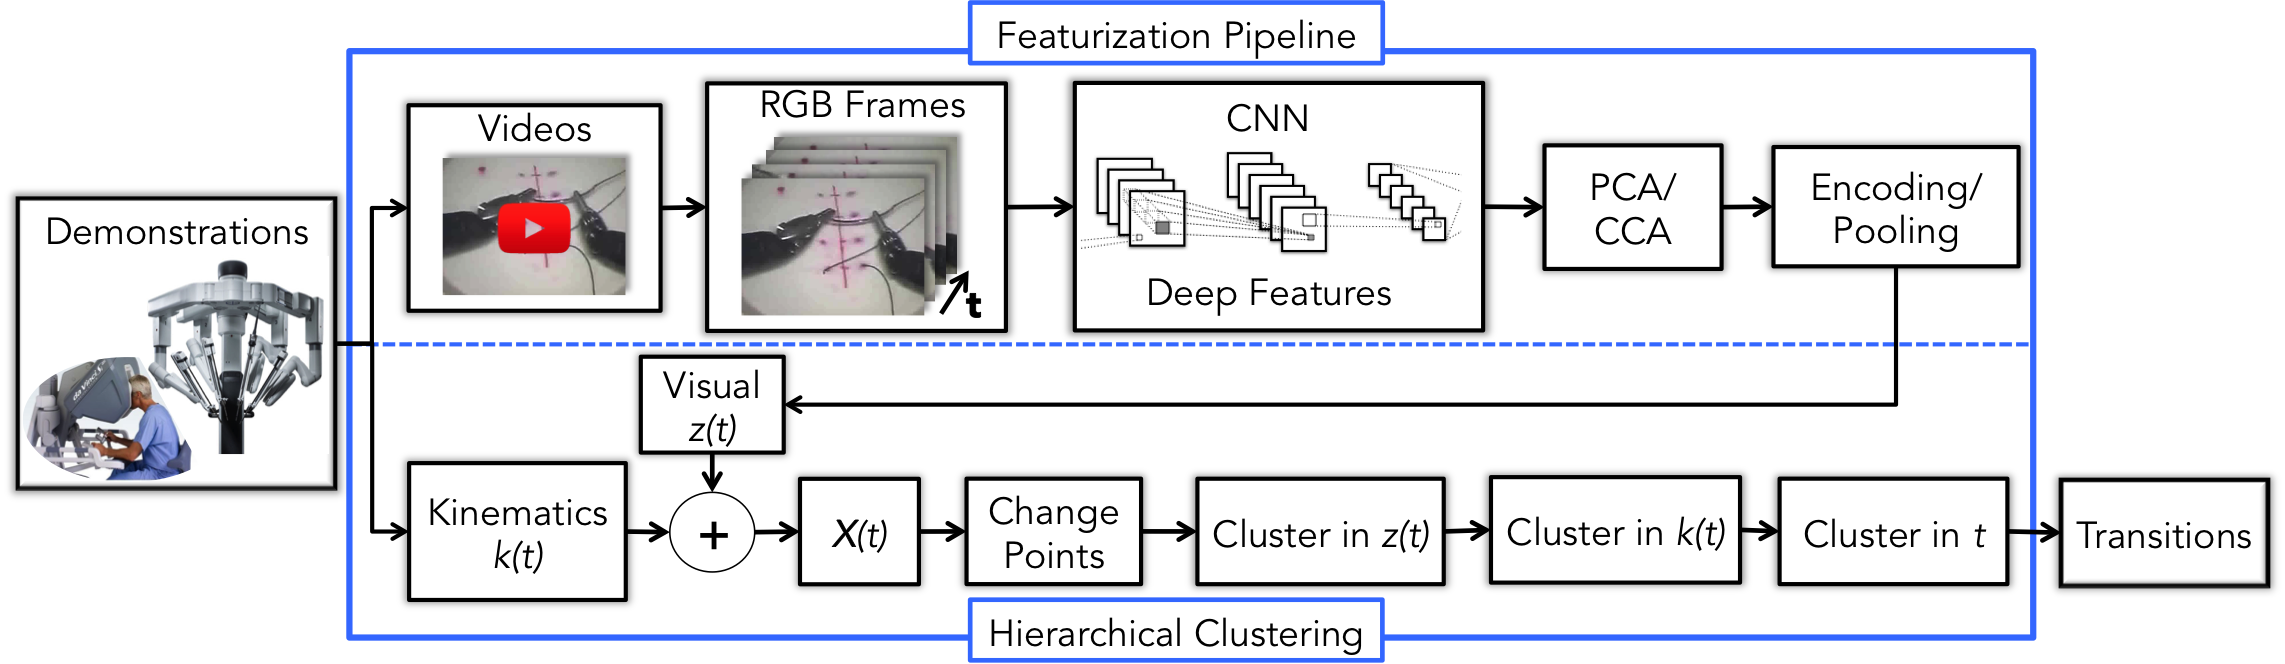
\includegraphics[width=0.8\linewidth]{figures/sysArch}
% \caption{\tsc is a task segmentation pipeline that starts with multimodal demonstrations (kinematics and vision), uses deep learning to featurize the frames of the video, and then clusters transition events to find segments.}
% \label{fig:pipeline}
% \vspace{-15pt}
% \end{figure*}

Unsupervised techniques can avoid dependence on a pre-defined set of primitives, and typically assume some generative mixture model for the data, e.g., locally Gaussian segments, and fit trajectories to this model grouping together locally similar points \cite{calinon2010learning, krishnan2015tsc, calinon2004stochastic, kruger2010learning, fox2009nonparametric, oh2005learning}.
While unsuperivsed segmentation has been widely studied in the context of kinematic data, increasingly, fixed camera video recordings accompany kinematic recordings of human tele-operation in a variety of datasets \cite{hodgins2009guide, gao2014jigsaws, ofli2013berkeley}.
Visual features can provide crucial information in a number of scenarios: (1) a robot can only partially observe its state with kinematic data, (2) state-dependent sensor noise in a robots kinematic data, and (3) manipulations of objects in the environment.
When they do use visual features, existing unsupervised approaches rely on highly constrained/feature-engineered visual sensing models: hand tuned features \cite{krishnan2015tsc}, poses for all objects in the workspace via AR markers \cite{Niekum2015learning}, or motion capture markers in human gesture extraction \cite{kulic2011incremental}.


In this work, we explore how we can relax these constraints by applying new results in Deep Learning.
In computer vision, the growing maturity of \emph{deep} featurization e.g., Convolutional Neural Networks (CNNs), has led to a number of seminal results in visual feature extraction \cite{krizhevsky2012imagenet, lecun1995convolutional, jia2014caffe, long2014fully}.
Furthermore, frameworks like CAFFE \cite{jia2014caffe} allow for sharing pre-trained models (on terabyte-scale corpora of natural images), and this allows us to take advantage of these results even with relatively small datasets.

We build on the Transition State Clustering algorithm \cite{krishnan2015tsc} and augment this model with task-agnostic visual features using Deep CNNs.
In our prior work, we proposed Transition State Clustering to segment demonstrations by learning switched linear dynamical systems and using clustering to identify regions of the state-space associated with switching events.
This algorithm applied a Dirichlet Process Gaussian mixture hierarchically first clustering transition states spatially and then temporally.
Our prior results suggested that augmenting the state-space with hand-tuned visual features could significantly improve accuracy of the learned ``transition state clusters".
In this work, we \emph{automatically} construct visual features using pre-trained CNNs applied to frames of video recordings; thus constructing a high-dimensional trajectory that augments the kinematic state-space.

\noindent We summarize the key experimental results:

\noindent\textbf{Featurization: } We evaluated 7 different visual featurization techniques, and our experimental results suggest high sensitivity to the choice of featurization with a 44\% variation in cluster tightness over the design space. Our results suggest that the conv5\_3 layer of the VGG architecture gives the tightest clustering performance \cite{simonyan2014very}.

\vspace{0.25em}
\noindent\textbf{Manual Annotation: } We use a dynamic time warping-based metric to evaluate our approach against manual annotation by domain experts and find at most a 5\% error in segmentation precision.

\vspace{0.25em}
\noindent\textbf{Visual Features Only: } We apply \tsc to a scenario where kinematics data is unavailable a human demonstration of a task without a robot. We find that the segmentation of this visual data aligns to segmentation of kinesthetic demonstrations of the same task with the PR2 with \todo{x\%} accuracy.  

\iffalse
\begin{figure}[ht]
\centering
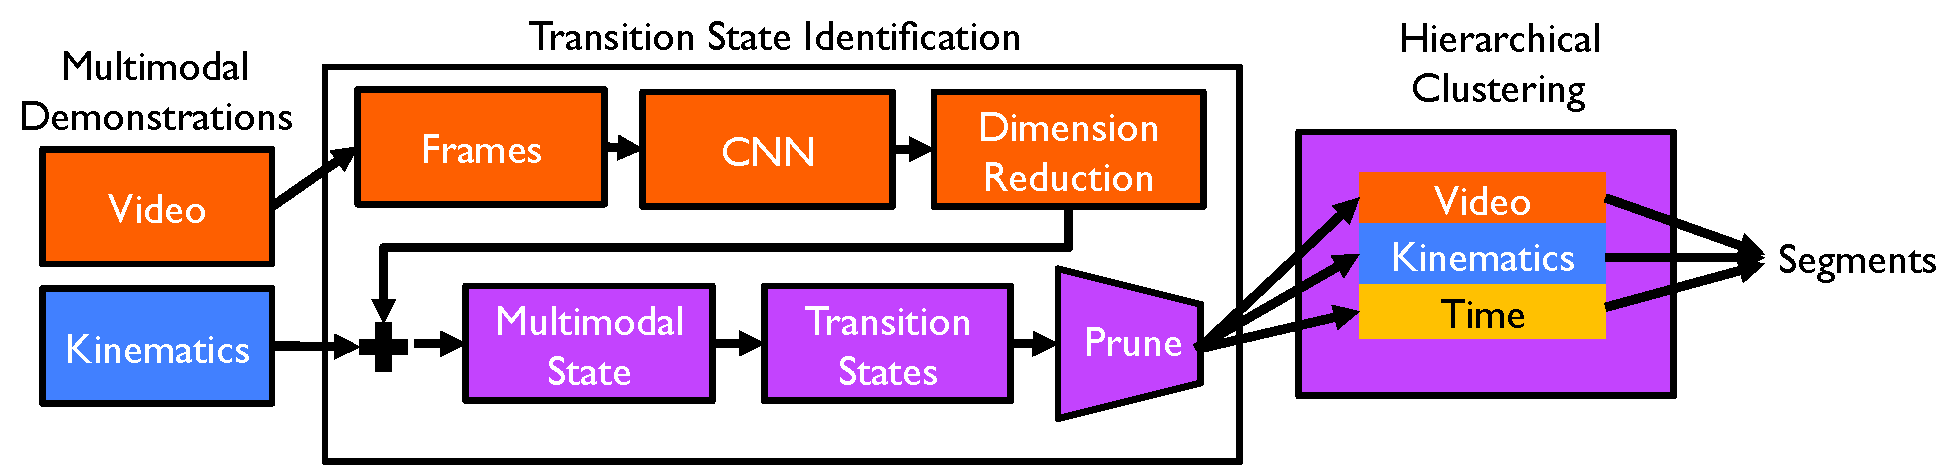
\includegraphics[width=\columnwidth]{figures/architecture.pdf}
\caption{\todo{name} architecture. We use a pre-trained CNN to featurize raw video data for use in segmentation. After featurization, we combine the data with kinematic data and apply a Transition State Clustering algorithm to identify segments.}
\figlabel{arch}
\vspace{-1em}
\end{figure}
\fi

\end{document}